\documentclass[border=4pt]{standalone}
\usepackage{tikz}
\usepackage{xcolor}
\usetikzlibrary{arrows.meta, positioning}
\newcommand{\pillar}[1]{\textcolor{blue!55!black}{\footnotesize\itshape #1}}
\begin{document}
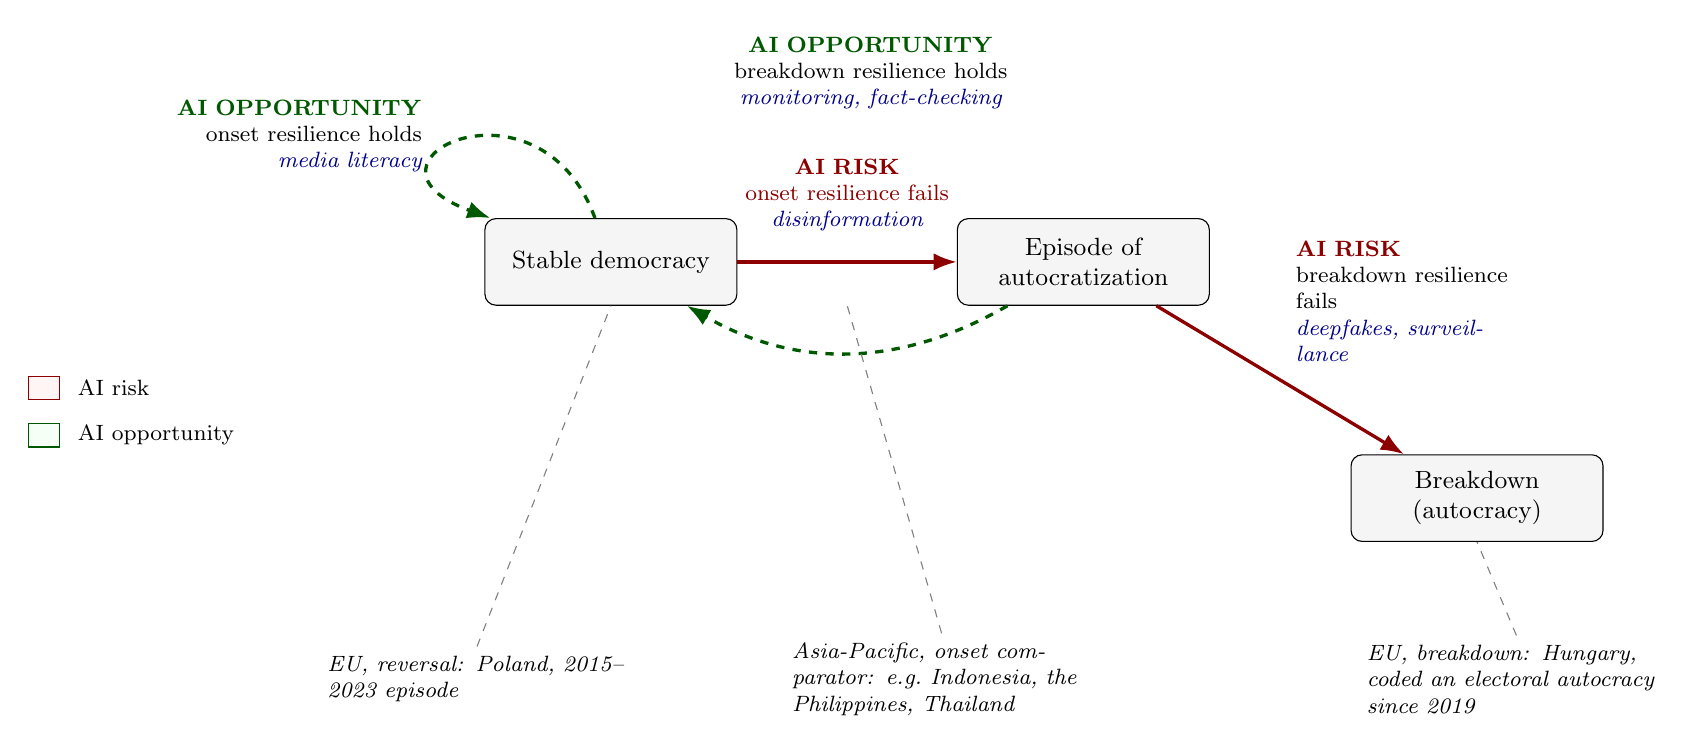
\begin{tikzpicture}[
  every node/.style = {font=\small},
  state/.style = {draw, rounded corners, align=center, minimum width=3.2cm, minimum height=1.1cm, fill=gray!8},
  lbl/.style = {font=\footnotesize\itshape, align=left, text width=3.8cm},
  tag/.style = {font=\footnotesize, align=center},
  conn/.style = {gray, dashed, -},
  >=Latex
]
  \node[state] (dem) at (0,5) {Stable democracy};
  \node[state] (epi) at (6,5) {Episode of\\autocratization};
  \node[state] (aut) at (11,2) {Breakdown\\(autocracy)};

  \draw[->, very thick, red!55!black] (dem) -- (epi);
  \node[tag, align=center, text width=3.2cm, red!55!black] at (3,5.85) {\textcolor{red!55!black}{\textbf{AI RISK}}\\onset resilience fails\\\pillar{disinformation}};

  \draw[->, very thick, red!55!black] (epi) -- (aut);
  \node[tag, align=left, text width=2.8cm] at (10.1,4.5) {\textcolor{red!55!black}{\textbf{AI RISK}}\\breakdown resilience fails\\\pillar{deepfakes, surveillance}};

  \draw[->, very thick, green!35!black, dashed] (epi) to[bend left=30] (dem);
  \node[tag, align=center, text width=4.6cm] at (3.3,7.4) {\textcolor{green!35!black}{\textbf{AI OPPORTUNITY}}\\breakdown resilience holds\\\pillar{monitoring, fact-checking}};

  \draw[->, very thick, green!35!black, dashed] (dem) to[out=110,in=160,looseness=4] (dem);
  \node[tag, align=right, text width=3.4cm] at (-4.1,6.6) {\textcolor{green!35!black}{\textbf{AI OPPORTUNITY}}\\onset resilience holds\\\pillar{media literacy}};

  \node[lbl] (lp) at (-1.7,-0.3) {EU, reversal: Poland, 2015--2023 episode};
  \node[lbl] (ls) at (4.2,-0.3) {Asia-Pacific, onset comparator: e.g.\ Indonesia, the Philippines, Thailand};
  \node[lbl] (lh) at (11.5,-0.3) {EU, breakdown: Hungary, coded an electoral autocracy since 2019};

  \draw[conn] (lp.north) -- (dem.south);
  \draw[conn] (ls.north) -- (3,4.45);
  \draw[conn] (lh.north) -- (aut.south);

  \node[draw=red!55!black, fill=red!4, minimum width=0.4cm, minimum height=0.3cm] (legr) at (-7.2,3.4) {};
  \node[right=0.1cm of legr, font=\footnotesize] {AI risk};
  \node[draw=green!35!black, fill=green!4, minimum width=0.4cm, minimum height=0.3cm] (lego) at (-7.2,2.8) {};
  \node[right=0.1cm of lego, font=\footnotesize] {AI opportunity};
\end{tikzpicture}
\end{document}
